
% !TeX spellcheck = nb_NB-NorwegianBokmal
\documentclass[10pt,aspectratio=169]{beamer}
\useinnertheme[shadow=true]{rounded}
% Add extra packages here
\usepackage[norsk]{babel}
\usepackage[T1]{fontenc}
\usepackage{amsmath}
\usepackage{graphicx}
\usepackage{tikz}  
\usepackage{chronosys}
\usepackage{tabularx}
\usepackage{svg}
%\usepackage{enumitem} 
\usepackage{comment}
\usetheme{_HK}

%\setsvg{inkscape = "C:/Program Files/Inkscape/inkscape.exe" -z -D}

\graphicspath{{figs/}}
% \usetheme{mc}
%
\title{Mørkfoss-Solbergfoss}
\subtitle{En kritisk brikke i utviklingen av norsk vannkraftteknologi}
\author{Bjarne B{\o}rresen}
\date{8. sep 2026}
\logo{
\includegraphics[width=3cm]{Hafslund_logo}}
%\titlegraphic{\includegraphics[width=0.2\textwidth]{ps_frontpage}}

\begin{document}
	%
\begin{frame}
	\titlepage
\end{frame}
%
\begin{frame}{Mørkfoss-Solbergfoss}
	\begin{columns}
		% Left Column
		\begin{column}{0.5\textwidth}
			\textbf{Plan}
			\begin{itemize}
				\item Historisk bakgrunn
				\item Aktiv industripolitikk
				\item Resultatet
			\end{itemize}
		\end{column}
		% Right Column
		\begin{column}{0.5\textwidth}
			\begin{center}
				% Replace 'example-image' with your actual file name
				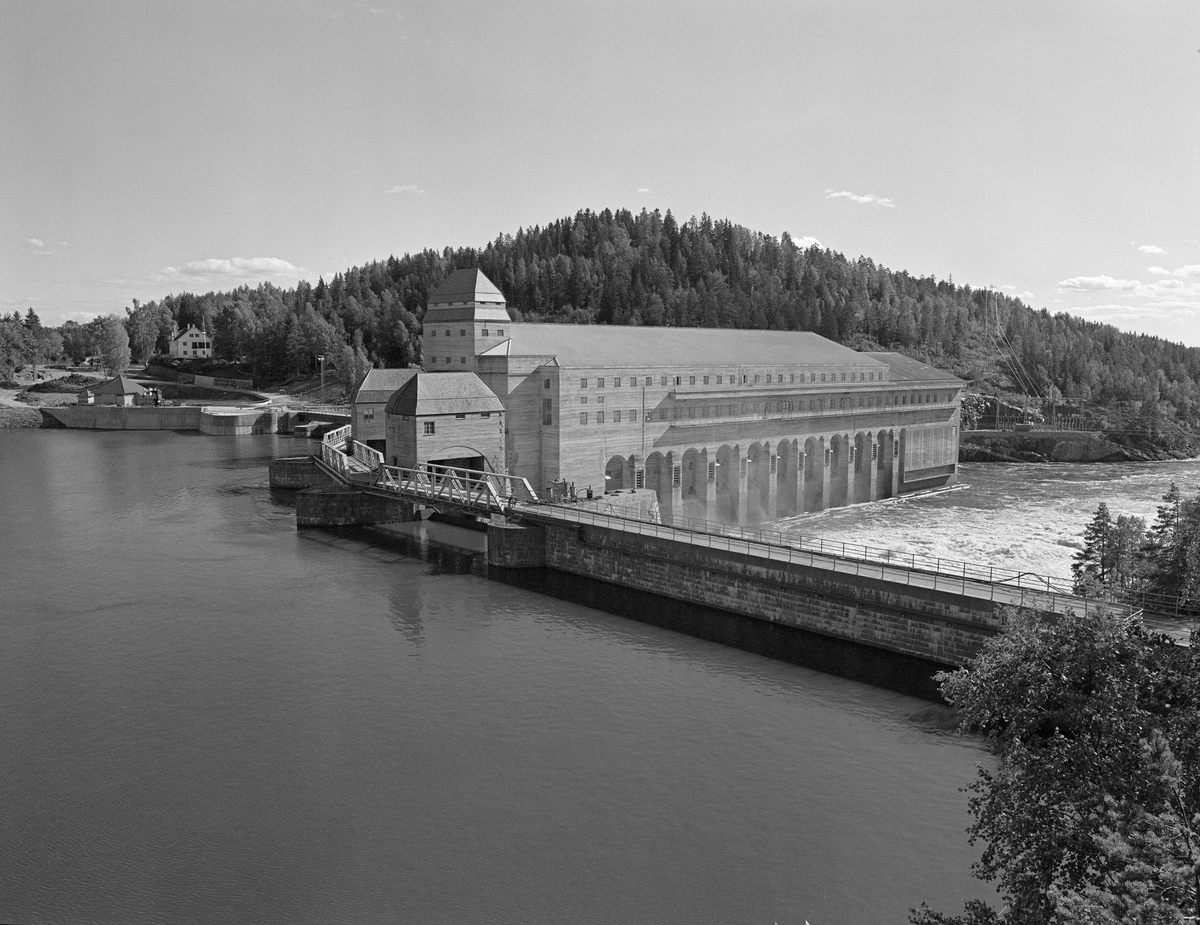
\includegraphics[width=\textwidth]{Solbergfoss_stasjon}
			\end{center}
		\end{column}
	\end{columns}
\end{frame}
%

\begin{frame}{Norsk vannkraftindustri før 1914}
%
\begin{columns}
	% Left Column
	\begin{column}{0.5\textwidth}
		\textbf{Store norske turbinleveranser:}
		\begin{tabular}{|c|c|c|c|} \hline
			Årstall & Anlegg & Effekt & Leverandør \\ \hline
			1900 & Hammeren &  6 x 420 kW & Myrens verksted  \\ \hline
			1901 & Øvre Lerfoss & 2 x 700 kW & Kværner Brug \\ \hline
		\end{tabular}
	\end{column}
	% Right Column
	\begin{column}{0.5\textwidth}
		\begin{center}
			% Replace 'example-image' with your actual file name
			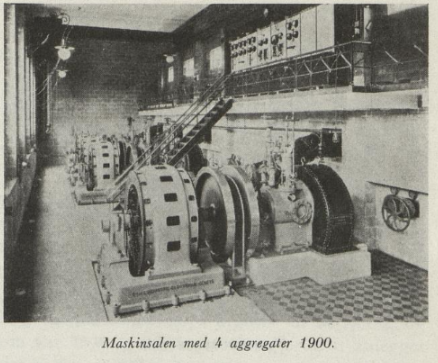
\includegraphics[width=0.5\textwidth]{Fig10_Hammern_1900}
		\end{center}
	\end{column}
\end{columns}

%
\vspace{0.1cm} % Space between top columns and bottom block


\startchronology[startyear=1880,stopyear=1930,color=HK_light_green, height=1cm, align=left]
\chronoevent{1885}{\rotatebox{-60}{Laugstol Brug}}
%\chronoevent[year=false]{1891}{\rotatebox{-60}{Hammerfest}}
\chronoevent{1892}{\rotatebox{-60}{Oslo Elektrisitetsverk}}
\chronoevent{1900}{\rotatebox{-60}{Hammern kraftverk}}
\chronoevent{1906}{\rotatebox{-60}{Panikkloven}}
\chronoevent{1910}{\rotatebox{-60}{NTH åpner}}
\chronoevent{1917}{\rotatebox{-60}{Vannkraftlaboratoriet}}
\chronoevent{1924}{\rotatebox{-60}{Solbergfoss åpner}}
\stopchronology

\end{frame}
%  
\begin{frame}{Etablering av NTH}
	\begin{columns}
		% Left Column
		\begin{column}{0.5\textwidth}
		\begin{center}
			% Replace 'example-image' with your actual file name
			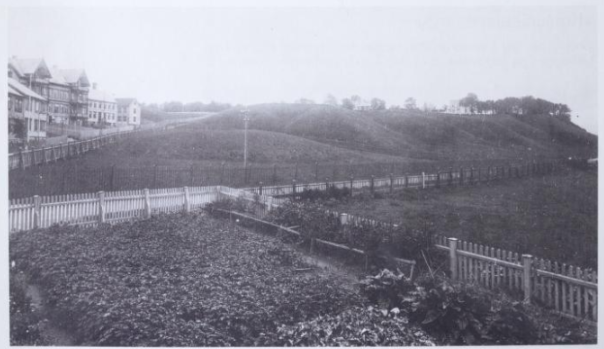
\includegraphics[width=0.9\textwidth]{Fig11b_Gloshaugen}
		\end{center}
		\end{column}
		% Right Column
		\begin{column}{0.5\textwidth}
			\textbf{15. september 1910}
			\begin{center}
				% Replace 'example-image' with your actual file name
				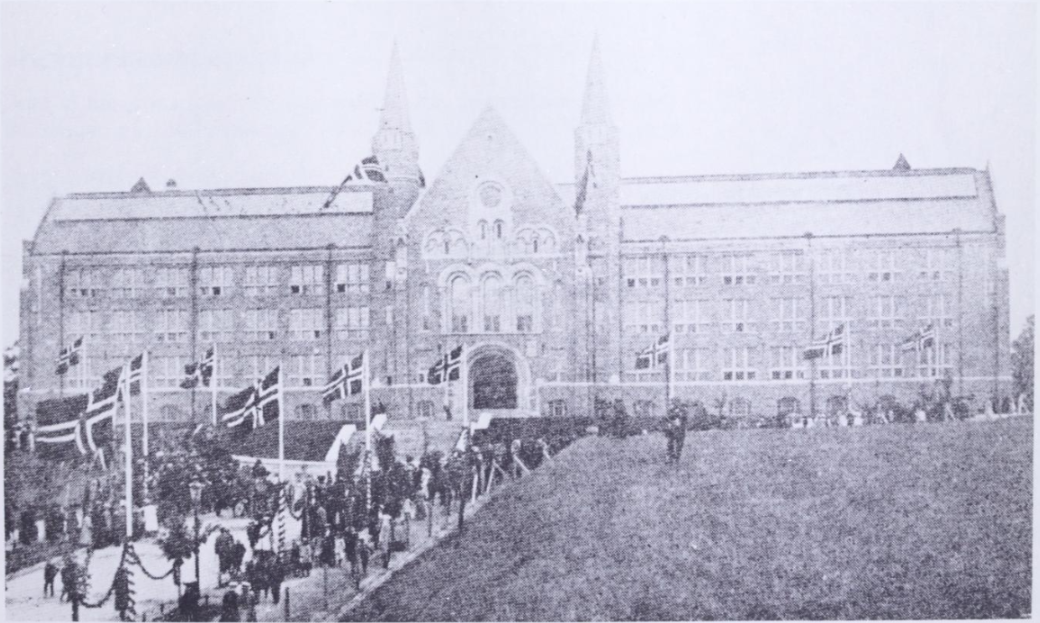
\includegraphics[width=0.9\textwidth]{Fig11_NTH}
			\end{center}
		\end{column}
	\end{columns}
\end{frame}
%
\begin{frame}{Professor Gudmund Sundby}
\begin{columns}
% Left Column
\begin{column}{0.5\textwidth}
	\textbf{Curiculum vitae:}
	\begin{itemize}
		\item 1898, Kristiania tekniske skole
		\item 1898-1912, Kværner Brug
		\item 1912, professor i vannkraftmaskiner ved NTH
	\end{itemize}
\end{column}
% Right Column
\begin{column}{0.5\textwidth}
	\begin{center}
		% Replace 'example-image' with your actual file name
		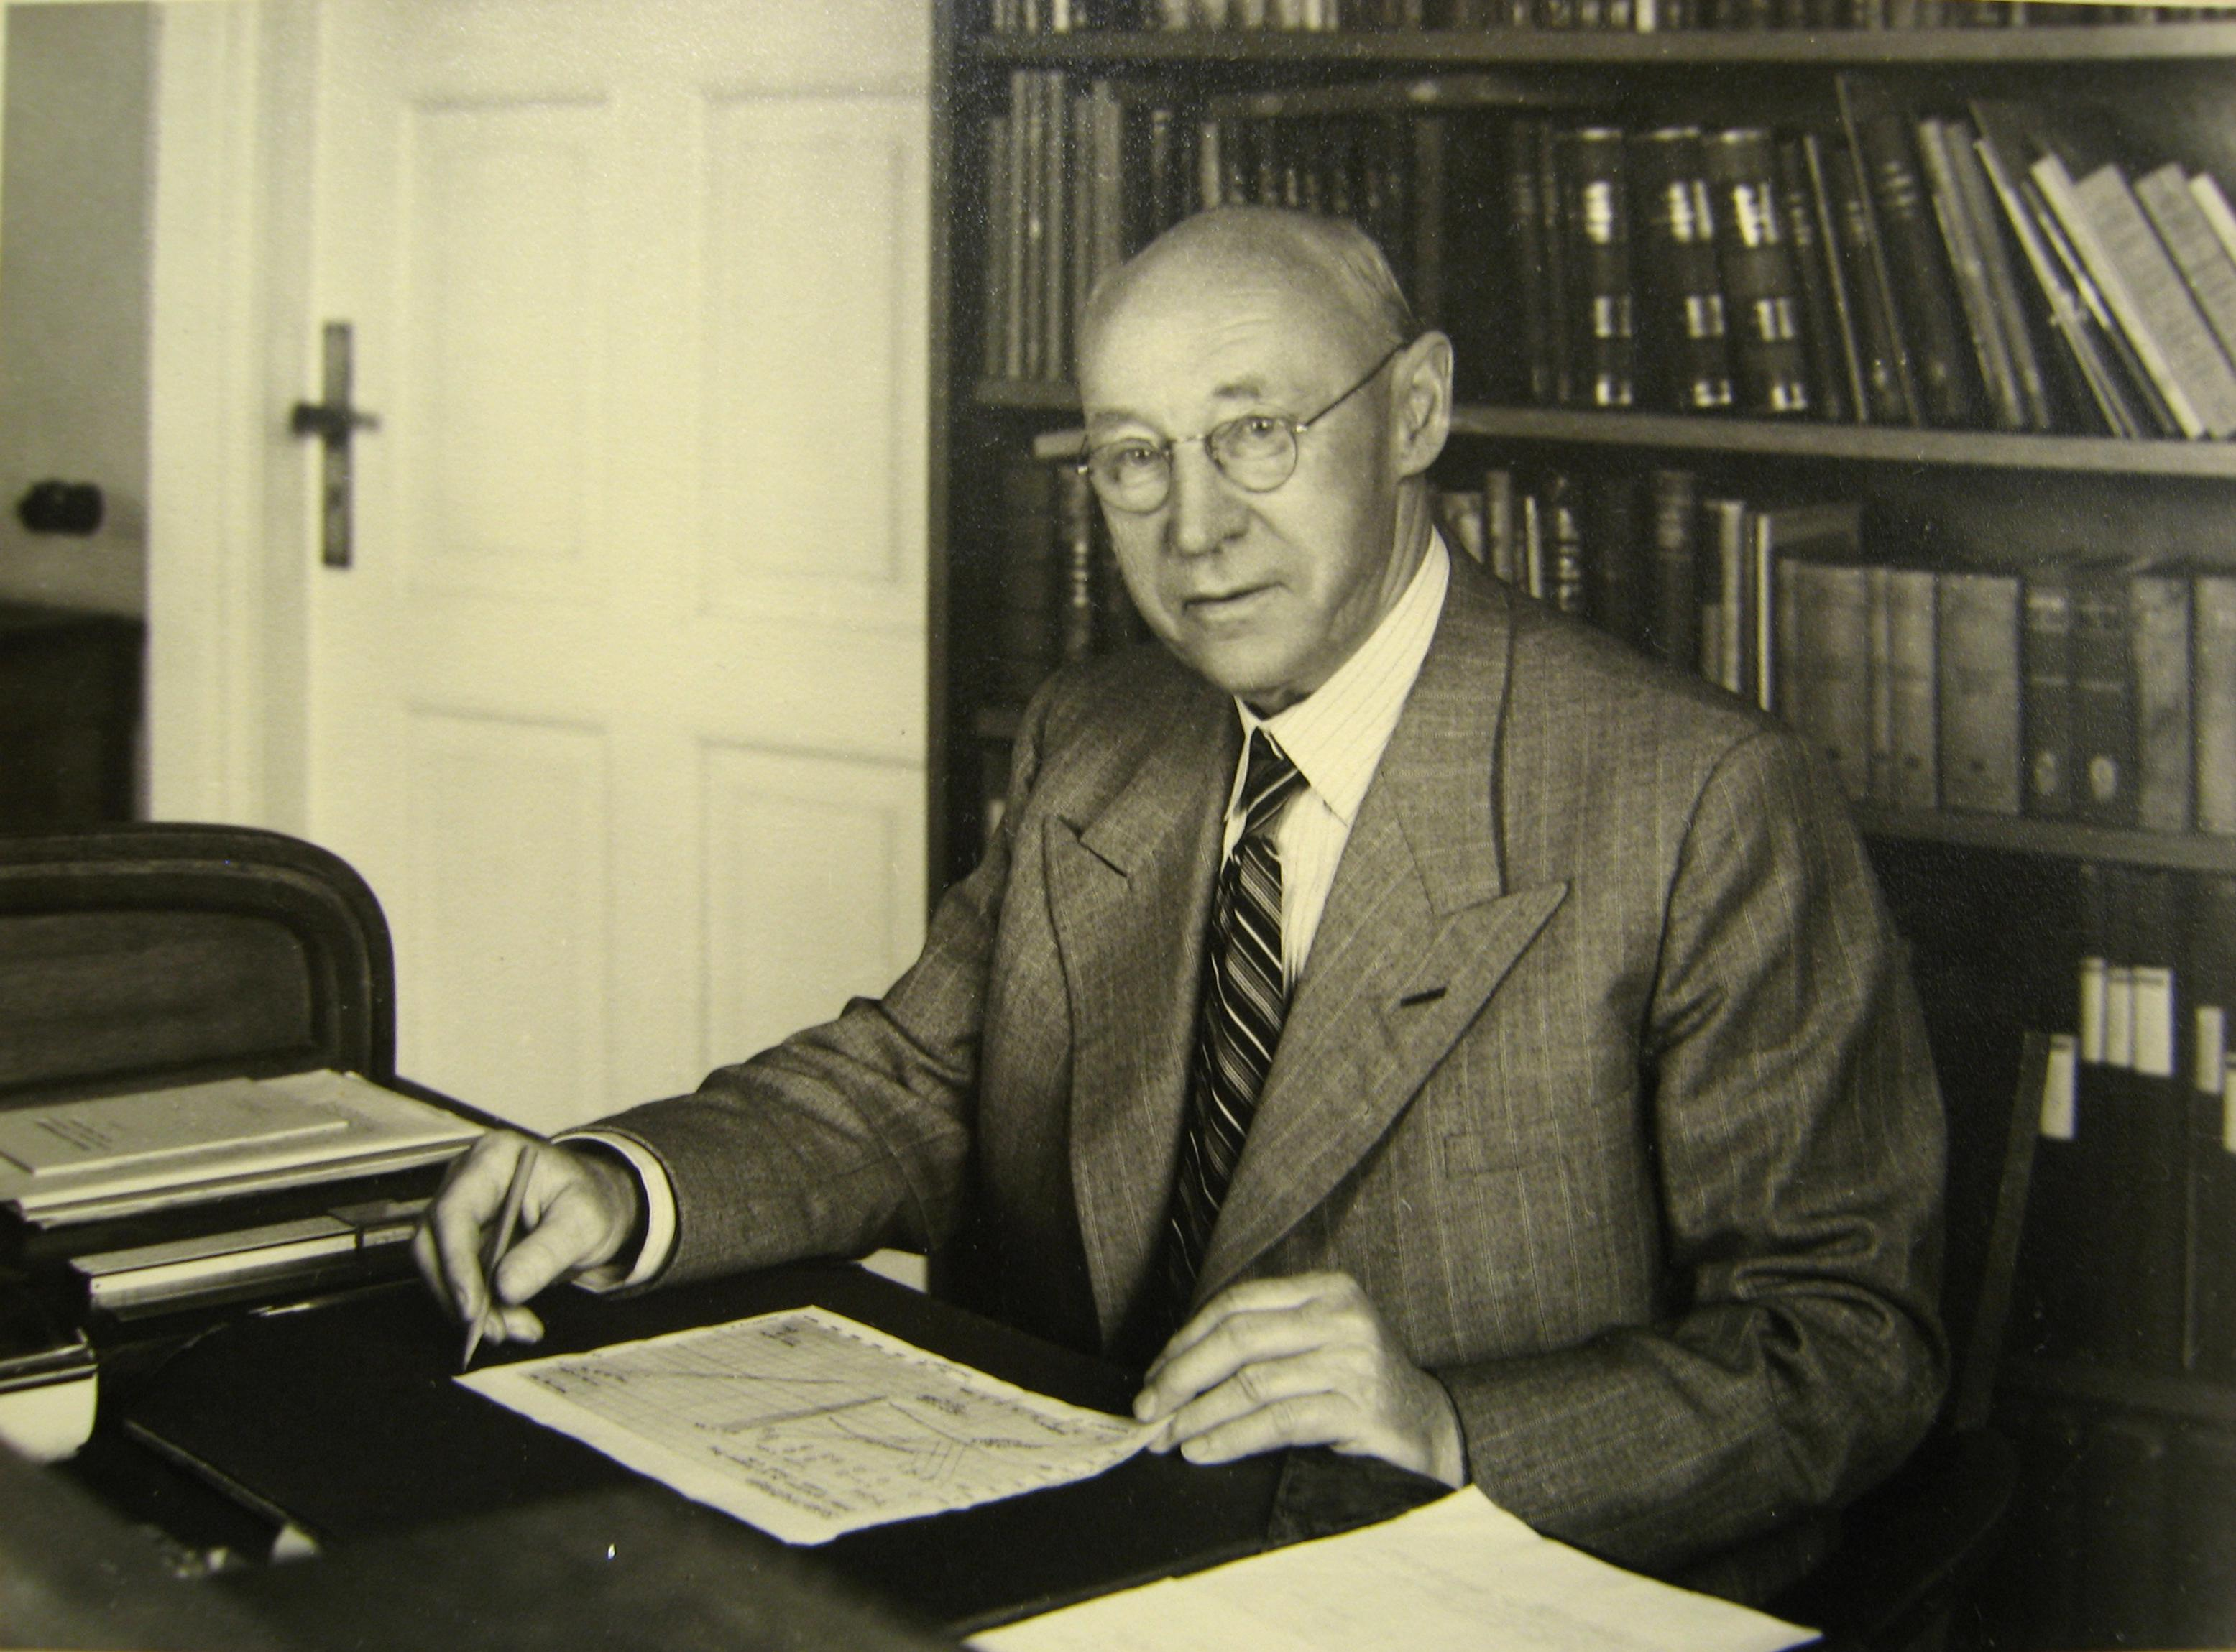
\includegraphics[width=0.9\textwidth]{fig03_Sundby}
	\end{center}
\end{column}
\end{columns}
\end{frame}
%
\begin{frame}{Statsminister Gunnar Knudsen}
	\begin{columns}
		% Left Column
		\begin{column}{0.5\textwidth}
			\textbf{Curiculum vitae:}
			\begin{itemize}
				\item 1869, Chalmerska Institutet i Göteborg
				\item 1885, Laugstol Bruks, første elektrisitetsverk
				\item 1908-1910, statsminister
				\item 1913-1920, 2. periode
			\end{itemize}
		\end{column}
		% Right Column
		\begin{column}{0.5\textwidth}
			\begin{center}
				% Replace 'example-image' with your actual file name
				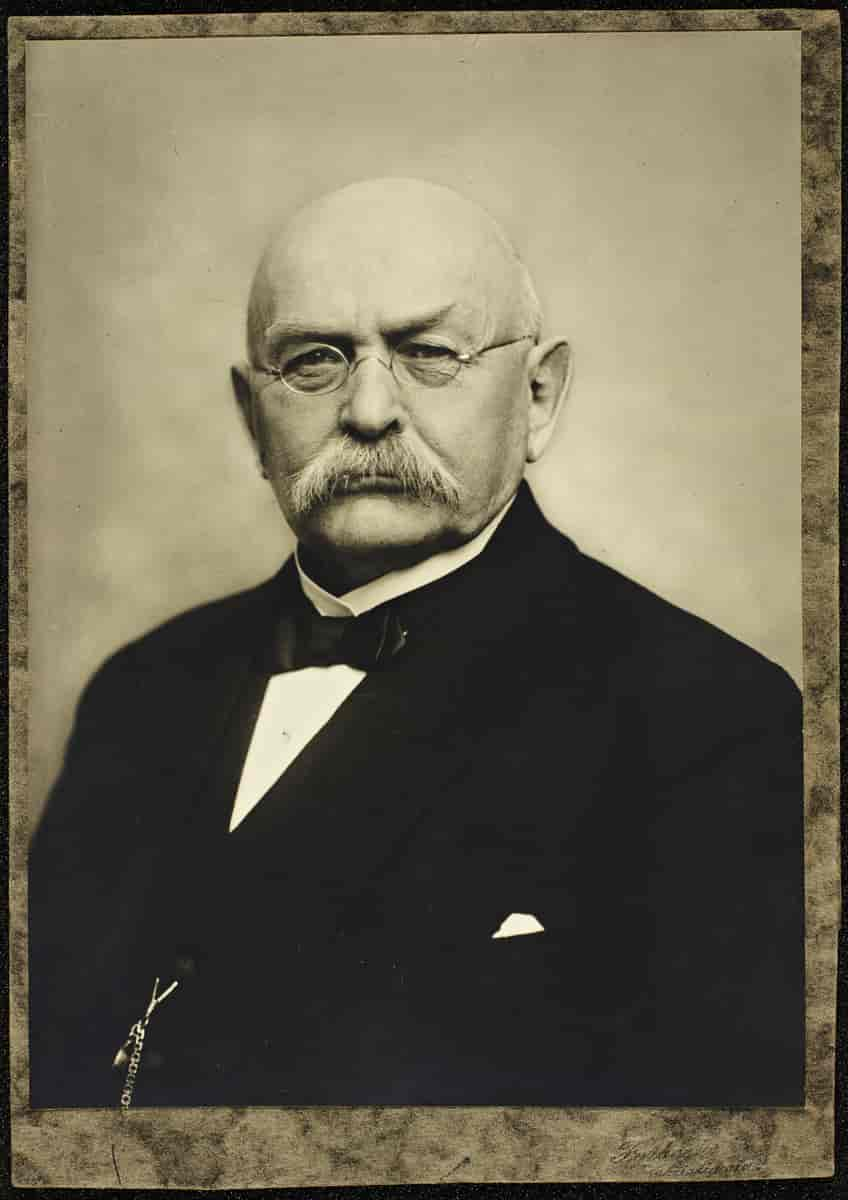
\includegraphics[width=0.9\textwidth]{fig04_Gunnar_Knudsen}
			\end{center}
		\end{column}
	\end{columns}
\end{frame}
%
\begin{frame}{Vannkraftlaboratoriet}
	\begin{columns}
		% Left Column
		\begin{column}{0.5\textwidth}
			\begin{center}
				% Replace 'example-image' with your actual file name
				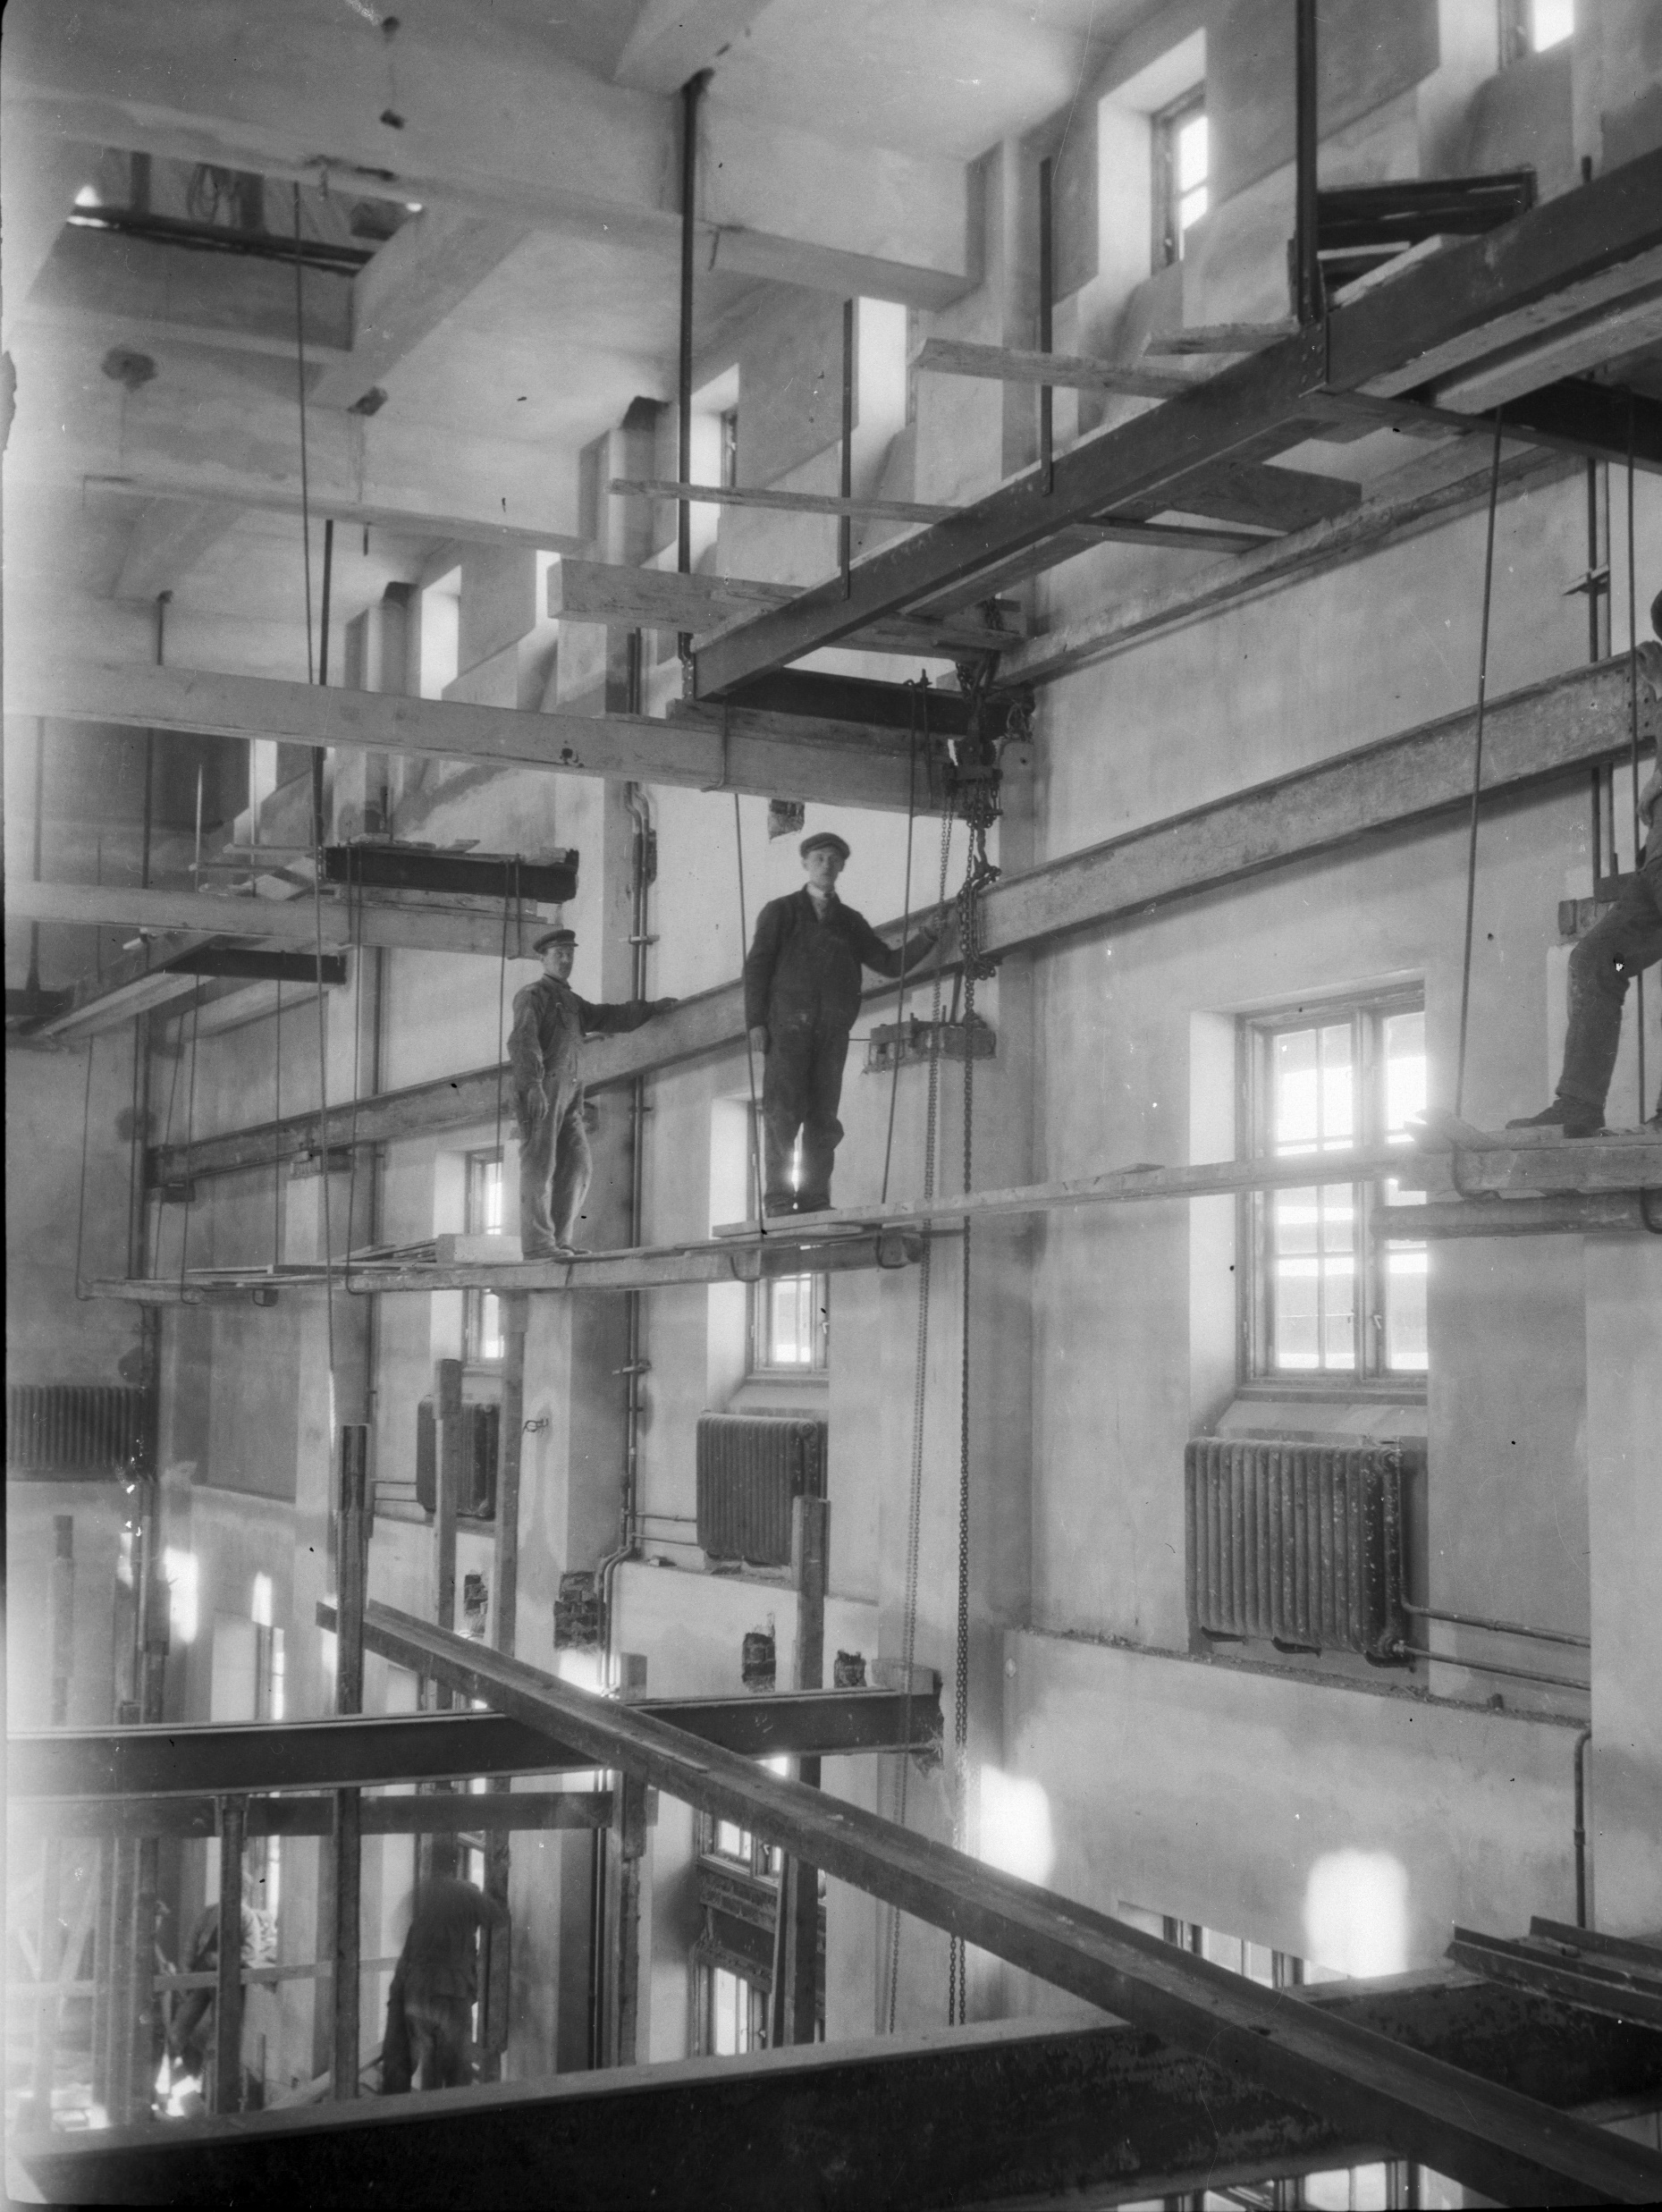
\includegraphics[width=0.8\textwidth]{fig06_VKLab02}
			\end{center}
		\end{column}
		% Right Column
		\begin{column}{0.5\textwidth}
			\begin{center}
				% Replace 'example-image' with your actual file name
				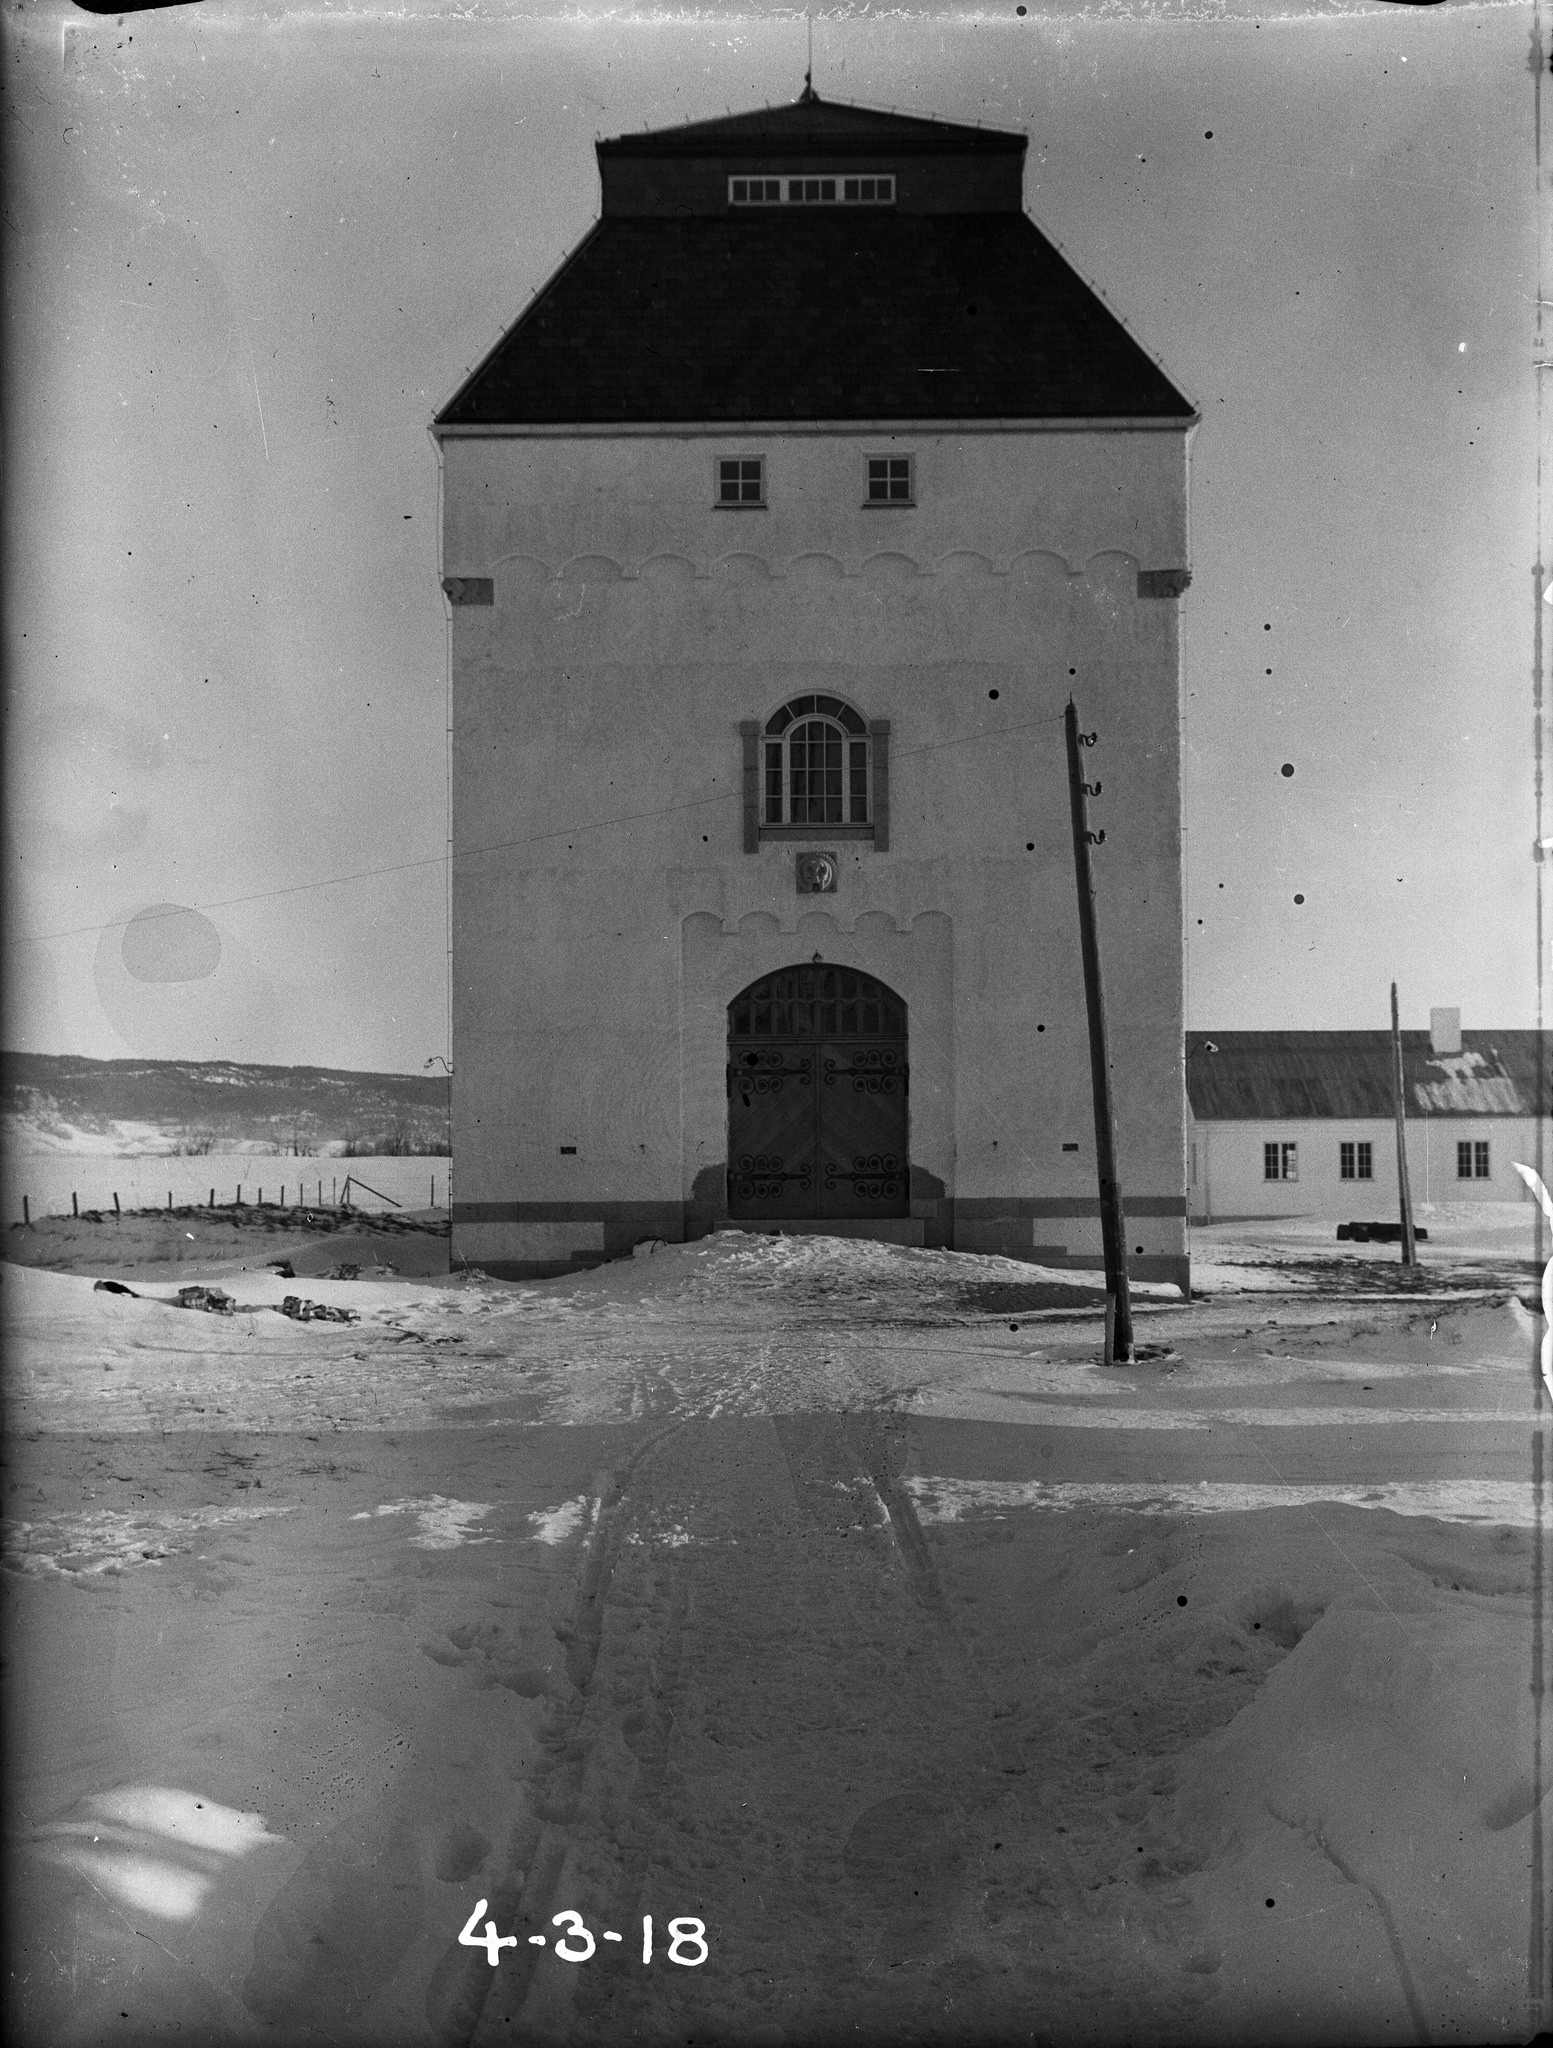
\includegraphics[width=0.8\textwidth]{fig05_VKLab01}
			\end{center}
		\end{column}
	\end{columns}
\end{frame}
%
\begin{frame}{Solbergfoss}
		\begin{columns}
		% Left Column
		\begin{column}{0.5\textwidth}
			\begin{center}
				% Replace 'example-image' with your actual file name
				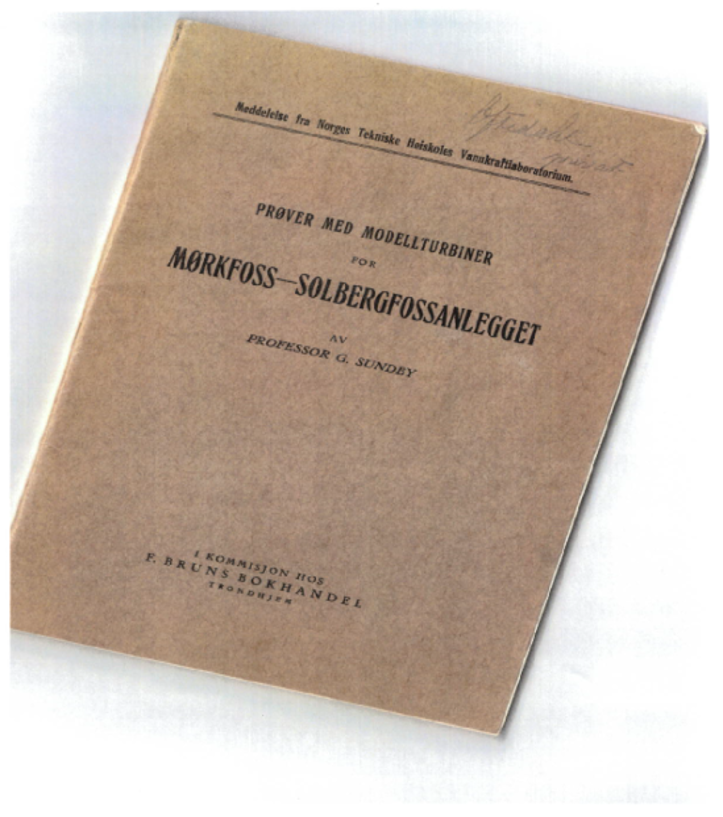
\includegraphics[width=0.8\textwidth]{Morkfoss_Solberfoss_mod_rapport}
			\end{center}
		\end{column}
		% Right Column
		\begin{column}{0.5\textwidth}
			\begin{center}
				% Replace 'example-image' with your actual file name
				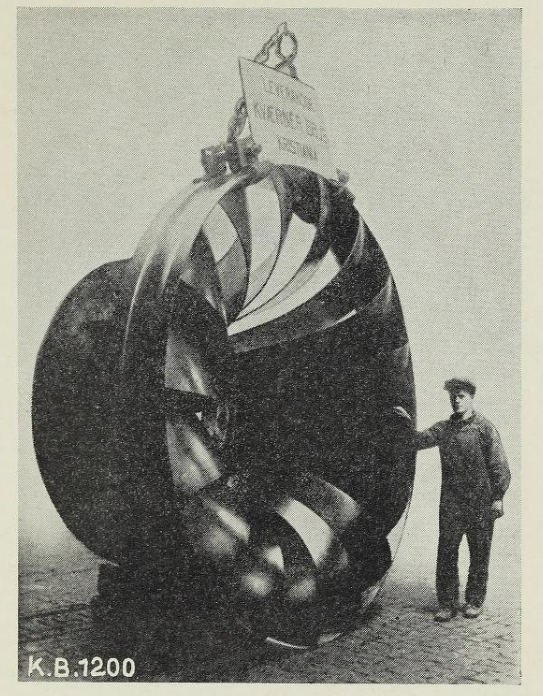
\includegraphics[width=0.8\textwidth]{Fig09_Lopehjul}
			\end{center}
		\end{column}
	\end{columns}
\end{frame}
%
\begin{frame}{The rest is history....}
		\begin{columns}
		% Left Column
		\begin{column}{0.5\textwidth}
			\textbf{Curiculum vitae:}
			\begin{itemize}
				\item 1932, Nygård, H=225 m, P=8 MW
				\item 1953, Vinstra, H=440 m, P=50 MW
				\item 1993, Svartisen, H=585 m, P=350 MW
				\item 2003, Three Gorges, H=80,6 m, P=700 MW
			\end{itemize}
		\end{column}
		% Right Column
		\begin{column}{0.5\textwidth}
			\begin{center}
				% Replace 'example-image' with your actual file name
				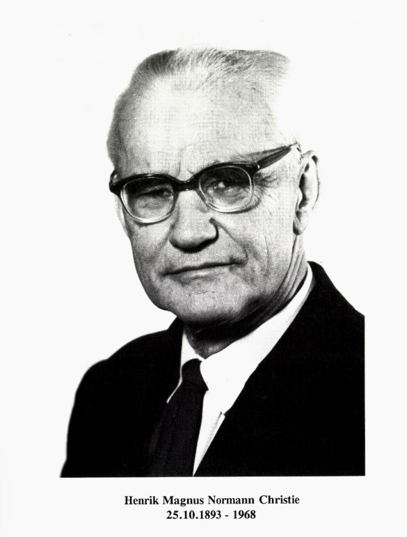
\includegraphics[width=0.5\textwidth]{Christie}\\ \vspace{0.5 cm}
				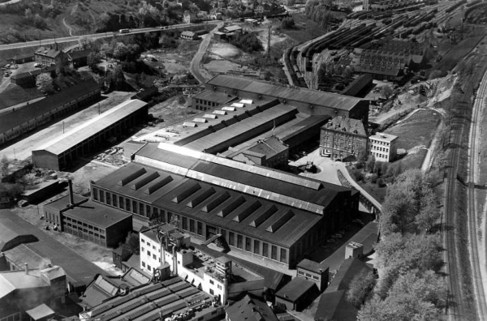
\includegraphics[width=0.5\textwidth]{Lodalen}
			\end{center}
		\end{column}
	\end{columns}
\end{frame}
%
\end{document}

